\section{Dawson's Chess on the Cylinder}\label{sec:dawson}

On a cylinder every file is alike, and the first move opens the ring of files into an ordinary strip. The
earlier study~\cite{Study2025} used this idea on Dawson's chess but stated the game incorrectly; here
we restate it and redo the analysis.

\begin{figure}[!t]
\centering
\begin{subfigure}{0.48\columnwidth}
\centering
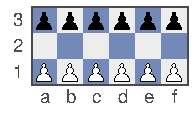
\includegraphics[scale=0.8]{figures/dawson_strip.pdf}
\caption{}
\label{fig:dawson_strip}
\end{subfigure}\hfill
\begin{subfigure}{0.48\columnwidth}
\centering
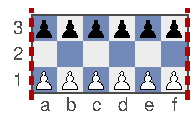
\includegraphics[scale=0.8]{figures/dawson_ring.pdf}
\caption{}
\label{fig:dawson_ring}
\end{subfigure}
\caption{Starting position of Dawson's chess on six files. (a) $3\times6$ ordinary board. (b) $3\times6$
cylinder: files a and f are adjacent; dashed edges are glued.}
\label{fig:dawson_boards}
\end{figure}

\begin{figure*}[!t]
\centering
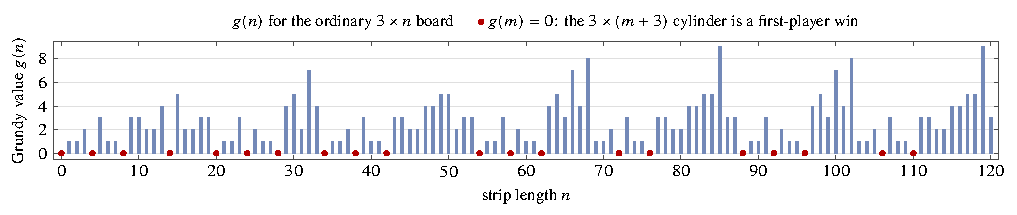
\includegraphics[width=\textwidth]{figures/dawson_grundy.pdf}
\caption{Grundy values $g(n)$ of Dawson's chess on the $3\times n$ ordinary board (octal game
$\mathbf{0.137}$), $n\le120$. Dots mark $g(m)=0$: the $3\times m$ board is a second-player win and the
$3\times(m+3)$ cylinder a first-player win (Theorem~\ref{thm:ring}).}
\label{fig:dawson_grundy}
\end{figure*}

\emph{Rules.} Dawson's chess~\cite{Dawson1935} is played on a $3\times n$ board
(Fig.~\ref{fig:dawson_boards}) with white pawns on rank~1, black pawns on rank~3 and rank~2 empty. Pawns move
and capture as in chess, captures are compulsory, and no pawn can double-step or promote. The last player to
move wins; in the mis\`ere form that Dawson posed, the last player loses.

Let us see what one move does. Call a file \emph{untouched} if both its pawns stand on their starting
squares. Suppose white plays c1--c2 with the b- and d-files untouched. The pawn on c2 attacks b3 and d3, so
black must capture, say b3$\times$c2. That pawn attacks b1 and d1, so white must recapture, say
d1$\times$c2, and then come d3$\times$c2 and b1$\times$c2. This leaves black to move, with the b- and
d-files empty and the c-file blocked for good, since a pawn enters a file only by capturing. At the end of a
row the push takes three plies and empties its one neighbor; a push with no untouched neighbor is
blocked.

Each such sequence is forced and touches only the pushed file and its neighbors. Counting a whole sequence as
one move, strips separated by empty files never interact, and both players have the same sequences, so this
game of sequences is impartial. A strip of $n$ untouched files is therefore the octal game $\mathbf{0.137}$~\cite{GuySmith1956,WinningWays},
in which a move removes a file and its untouched neighbors. Its Grundy values are $g(0)=0$, $g(1)=1$ and,
for $n\ge2$,
\begin{equation}\label{eq:dawson}
g(n)=\operatorname{mex}\bigl(\{g(n-2)\}\cup\{g(a)\oplus g(b) : a+b=n-3\}\bigr),
\end{equation}
where $a,b\ge0$, $\oplus$ is the nim-sum and mex is the least non-negative integer not in the set. The first
player wins the ordinary $3\times n$ board exactly when $g(n)\ne0$. The values from~\eqref{eq:dawson}
have period 34 with last exception $n=51$~\cite{GuySmith1956}, which two programs reproduce for $n\le300$
\lab{C2}.

\emph{What was wrong.} In~\cite{Study2025} a pawn could be removed from a single row only when
both its neighbors were empty, so a full row of two or more pawns has no move. Its recurrence lacks the
end-file term $g(n-2)$ of~\eqref{eq:dawson} and the value $g(1)=1$, agrees with $g$ at only 31 of the 301 values
$n\le300$, and gives the wrong cylinder outcome for 56 of them \lab{C2}. The first is $n=4$, a predicted
first-player win: white's push and four captures leave one untouched file, black pushes that pawn, it is
blocked, and white has no move.

\begin{theorem}[Ring rule; \lab{P}, machine-checked for $n\le22$]\label{thm:ring}
On the full $3\times n$ cylinder, $n\ge3$, every first move with its forced captures leaves one strip of
$n-3$ untouched files, with the opponent to move. Hence the cylinder has Grundy value
$\operatorname{mex}\{g(n-3)\}$, and the first player wins if and only if $g(n-3)=0$, that is, for
$n=3,7,11,17,23,27,31,37,41,45,57,\dots$
\end{theorem}

\begin{proof}
Every file of a full ring has two distinct untouched neighbors, so every push starts the five-ply sequence
above. The other $n-3$ files, bounded by empty files that never change, form an ordinary strip. By
rotation all first moves are alike, and the cylinder has one option.
\end{proof}

The ring formula of~\cite{Study2025} and its remark that the ring's value is always 0 or 1 are
right once the correct $g$ is used (Fig.~\ref{fig:dawson_grundy}).

\emph{Mis\`ere play.} A forced sequence has odd length and ends with the player who began it, so the
ring rule carries over: the first player wins the mis\`ere cylinder exactly when the strip of $n-3$ files is
a mis\`ere P-position. Our implementation of the Plambeck--Siegel algorithm~\cite{PlambeckSiegel2008}
reproduces their partial quotient for strips of at most 32 files (order 638, 109 P-positions) and agrees
with exhaustive search on 7.4 million positions \lab{C2}; our computation of the next quotient, for longer strips, did not finish.

\emph{A warning about sums.} As a partizan game on its own, the ordinary $3\times5$ board is $\star$,
although $g(5)=3$. The outcome agrees, but only $g$ adds up: a sum of such values would let a player reply
elsewhere while a capture is pending.
